\documentclass{extbook}[14pt]
\usepackage{multicol, enumerate, enumitem, hyperref, color, soul, setspace, parskip, fancyhdr, amssymb, amsthm, amsmath, latexsym, units, mathtools}
\everymath{\displaystyle}
\usepackage[headsep=0.5cm,headheight=0cm, left=1 in,right= 1 in,top= 1 in,bottom= 1 in]{geometry}
\usepackage{dashrule}  % Package to use the command below to create lines between items
\newcommand{\litem}[1]{\item #1

\rule{\textwidth}{0.4pt}}
\pagestyle{fancy}
\lhead{}
\chead{Answer Key for Module6 Version B}
\rhead{}
\lfoot{2107-1615}
\cfoot{}
\rfoot{test}
\begin{document}
\textbf{This key should allow you to understand why you choose the option you did (beyond just getting a question right or wrong). \href{https://xronos.clas.ufl.edu/mac1105spring2020/courseDescriptionAndMisc/Exams/LearningFromResults}{More instructions on how to use this key can be found here}.}

\textbf{If you have a suggestion to make the keys better, \href{https://forms.gle/CZkbZmPbC9XALEE88}{please fill out the short survey here}.}

\textit{Note: This key is auto-generated and may contain issues and/or errors. The keys are reviewed after each exam to ensure grading is done accurately. If there are issues (like duplicate options), they are noted in the offline gradebook. The keys are a work-in-progress to give students as many resources to improve as possible.}

\rule{\textwidth}{0.4pt}

\begin{enumerate}\litem{
Construct the lowest-degree polynomial given the zeros below. Then, choose the intervals that contain the coefficients of the polynomial in the form $x^3+bx^2+cx+d$.
\[ -4 + 5 i \text{ and } -3 \]The solution is \( x^{3} +11 x^{2} +65 x + 123 \), which is option B.\begin{enumerate}[label=\Alph*.]
\item \( b \in [-14, -10], c \in [63, 72], \text{ and } d \in [-129, -116] \)

$x^{3} -11 x^{2} +65 x -123$, which corresponds to multiplying out $(x-(-4 + 5 i))(x-(-4 - 5 i))(x -3)$.
\item \( b \in [7, 14], c \in [63, 72], \text{ and } d \in [119, 125] \)

* $x^{3} +11 x^{2} +65 x + 123$, which is the correct option.
\item \( b \in [1, 9], c \in [-5, 1], \text{ and } d \in [-24, -14] \)

$x^{3} + x^{2} -2 x -15$, which corresponds to multiplying out $(x -5)(x + 3)$.
\item \( b \in [1, 9], c \in [4, 13], \text{ and } d \in [11, 20] \)

$x^{3} + x^{2} +7 x + 12$, which corresponds to multiplying out $(x + 4)(x + 3)$.
\item \( \text{None of the above.} \)

This corresponds to making an unanticipated error or not understanding how to use nonreal complex numbers to create the lowest-degree polynomial. If you chose this and are not sure what you did wrong, please contact the coordinator for help.
\end{enumerate}

\textbf{General Comment:} Remember that the conjugate of $a+bi$ is $a-bi$. Since these zeros always come in pairs, we need to multiply out $(x-(-4 + 5 i))(x-(-4 - 5 i))(x-(-3))$.
}
\litem{
Construct the lowest-degree polynomial given the zeros below. Then, choose the intervals that contain the coefficients of the polynomial in the form $ax^3+bx^2+cx+d$.
\[ \frac{-5}{2}, \frac{-7}{4}, \text{ and } -2 \]The solution is \( 8x^{3} +50 x^{2} +103 x + 70 \), which is option B.\begin{enumerate}[label=\Alph*.]
\item \( a \in [3, 9], b \in [3, 13], c \in [-51, -46], \text{ and } d \in [-70, -67] \)

$8x^{3} +10 x^{2} -47 x -70$, which corresponds to multiplying out $(2x -5)(4x + 7)(x + 2)$.
\item \( a \in [3, 9], b \in [48, 52], c \in [97, 108], \text{ and } d \in [68, 74] \)

* $8x^{3} +50 x^{2} +103 x + 70$, which is the correct option.
\item \( a \in [3, 9], b \in [48, 52], c \in [97, 108], \text{ and } d \in [-70, -67] \)

$8x^{3} +50 x^{2} +103 x -70$, which corresponds to multiplying everything correctly except the constant term.
\item \( a \in [3, 9], b \in [-60, -47], c \in [97, 108], \text{ and } d \in [-70, -67] \)

$8x^{3} -50 x^{2} +103 x -70$, which corresponds to multiplying out $(2x -5)(4x -7)(x -2)$.
\item \( a \in [3, 9], b \in [-23, -17], c \in [-33, -29], \text{ and } d \in [68, 74] \)

$8x^{3} -18 x^{2} -33 x + 70$, which corresponds to multiplying out $(2x -5)(4x -7)(x + 2)$.
\end{enumerate}

\textbf{General Comment:} To construct the lowest-degree polynomial, you want to multiply out $(2x + 5)(4x + 7)(x + 2)$
}
\litem{
Describe the zero behavior of the zero $x = 5$ of the polynomial below.
\[ f(x) = 2(x - 7)^{10}(x + 7)^{8}(x - 5)^{8}(x + 5)^{3} \]The solution is the graph below, which is option C.
\begin{center}
    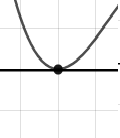
\includegraphics[width=0.3\textwidth]{../Figures/polyZeroBehaviorCB.png}
\end{center}\begin{enumerate}[label=\Alph*.]
\begin{multicols}{2}
\item 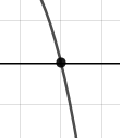
\includegraphics[width = 0.3\textwidth]{../Figures/polyZeroBehaviorAB.png}
\item 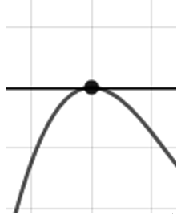
\includegraphics[width = 0.3\textwidth]{../Figures/polyZeroBehaviorBB.png}
\item 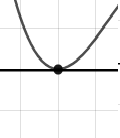
\includegraphics[width = 0.3\textwidth]{../Figures/polyZeroBehaviorCB.png}
\item 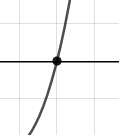
\includegraphics[width = 0.3\textwidth]{../Figures/polyZeroBehaviorDB.png}
\end{multicols}\item None of the above.\end{enumerate}
\textbf{General Comment:} You will need to sketch the entire graph, then zoom in on the zero the question asks about.
}
\litem{
Describe the zero behavior of the zero $x = 5$ of the polynomial below.
\[ f(x) = -4(x + 4)^{8}(x - 4)^{7}(x - 5)^{9}(x + 5)^{4} \]The solution is the graph below, which is option A.
\begin{center}
    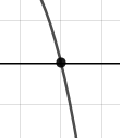
\includegraphics[width=0.3\textwidth]{../Figures/polyZeroBehaviorCopyAB.png}
\end{center}\begin{enumerate}[label=\Alph*.]
\begin{multicols}{2}
\item 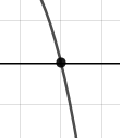
\includegraphics[width = 0.3\textwidth]{../Figures/polyZeroBehaviorCopyAB.png}
\item 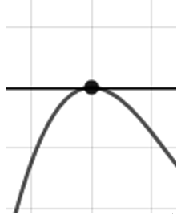
\includegraphics[width = 0.3\textwidth]{../Figures/polyZeroBehaviorCopyBB.png}
\item 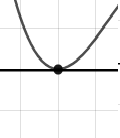
\includegraphics[width = 0.3\textwidth]{../Figures/polyZeroBehaviorCopyCB.png}
\item 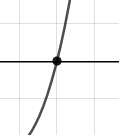
\includegraphics[width = 0.3\textwidth]{../Figures/polyZeroBehaviorCopyDB.png}
\end{multicols}\item None of the above.\end{enumerate}
\textbf{General Comment:} You will need to sketch the entire graph, then zoom in on the zero the question asks about.
}
\litem{
Which of the following equations \textit{could} be of the graph presented below?

\begin{center}
    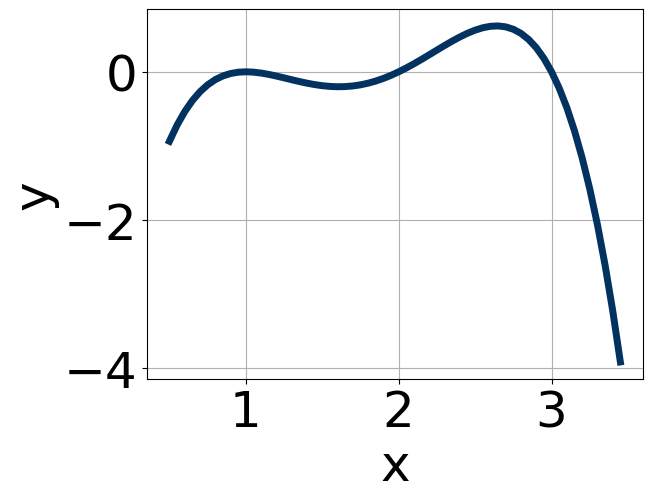
\includegraphics[width=0.5\textwidth]{../Figures/polyGraphToFunctionCopyB.png}
\end{center}


The solution is \( -11(x - 3)^{11} (x - 2)^{5} (x + 4)^{9} \), which is option C.\begin{enumerate}[label=\Alph*.]
\item \( 6(x - 3)^{8} (x - 2)^{7} (x + 4)^{5} \)

The factor $(x - 3)$ should have an odd power and the leading coefficient should be the opposite sign.
\item \( -9(x - 3)^{8} (x - 2)^{10} (x + 4)^{7} \)

The factors $3$ and $2$ have have been odd power.
\item \( -11(x - 3)^{11} (x - 2)^{5} (x + 4)^{9} \)

* This is the correct option.
\item \( -5(x - 3)^{10} (x - 2)^{7} (x + 4)^{7} \)

The factor $3$ should have been an odd power.
\item \( 19(x - 3)^{7} (x - 2)^{9} (x + 4)^{5} \)

This corresponds to the leading coefficient being the opposite value than it should be.
\end{enumerate}

\textbf{General Comment:} General Comments: Draw the x-axis to determine which zeros are touching (and so have even multiplicity) or cross (and have odd multiplicity).
}
\litem{
Describe the end behavior of the polynomial below.
\[ f(x) = 8(x + 8)^{2}(x - 8)^{3}(x + 4)^{5}(x - 4)^{5} \]The solution is the graph below, which is option D.
\begin{center}
    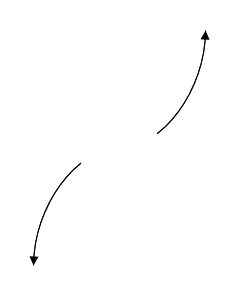
\includegraphics[width=0.3\textwidth]{../Figures/polyEndBehaviorDB.png}
\end{center}\begin{enumerate}[label=\Alph*.]
\begin{multicols}{2}
\item 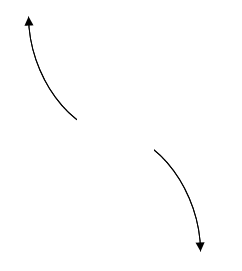
\includegraphics[width = 0.3\textwidth]{../Figures/polyEndBehaviorAB.png}
\item 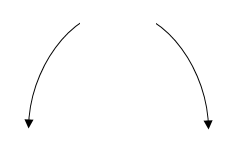
\includegraphics[width = 0.3\textwidth]{../Figures/polyEndBehaviorBB.png}
\item 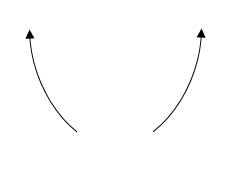
\includegraphics[width = 0.3\textwidth]{../Figures/polyEndBehaviorCB.png}
\item 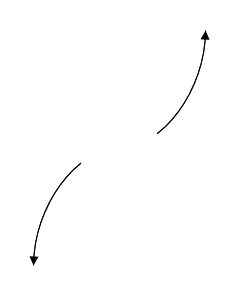
\includegraphics[width = 0.3\textwidth]{../Figures/polyEndBehaviorDB.png}
\end{multicols}\item None of the above.\end{enumerate}
\textbf{General Comment:} Remember that end behavior is determined by the leading coefficient AND whether the \textbf{sum} of the multiplicities is positive or negative.
}
\litem{
Construct the lowest-degree polynomial given the zeros below. Then, choose the intervals that contain the coefficients of the polynomial in the form $x^3+bx^2+cx+d$.
\[ 3 - 5 i \text{ and } -4 \]The solution is \( x^{3} -2 x^{2} +10 x + 136 \), which is option B.\begin{enumerate}[label=\Alph*.]
\item \( b \in [0.96, 1.62], c \in [7.42, 9.73], \text{ and } d \in [17, 22] \)

$x^{3} + x^{2} +9 x + 20$, which corresponds to multiplying out $(x + 5)(x + 4)$.
\item \( b \in [-2.98, -1.83], c \in [9.75, 11.93], \text{ and } d \in [132, 142] \)

* $x^{3} -2 x^{2} +10 x + 136$, which is the correct option.
\item \( b \in [1.06, 2.5], c \in [9.75, 11.93], \text{ and } d \in [-137, -131] \)

$x^{3} +2 x^{2} +10 x -136$, which corresponds to multiplying out $(x-(3 - 5 i))(x-(3 + 5 i))(x -4)$.
\item \( b \in [0.96, 1.62], c \in [0.77, 1.03], \text{ and } d \in [-18, -5] \)

$x^{3} + x^{2} +x -12$, which corresponds to multiplying out $(x -3)(x + 4)$.
\item \( \text{None of the above.} \)

This corresponds to making an unanticipated error or not understanding how to use nonreal complex numbers to create the lowest-degree polynomial. If you chose this and are not sure what you did wrong, please contact the coordinator for help.
\end{enumerate}

\textbf{General Comment:} Remember that the conjugate of $a+bi$ is $a-bi$. Since these zeros always come in pairs, we need to multiply out $(x-(3 - 5 i))(x-(3 + 5 i))(x-(-4))$.
}
\litem{
Construct the lowest-degree polynomial given the zeros below. Then, choose the intervals that contain the coefficients of the polynomial in the form $ax^3+bx^2+cx+d$.
\[ 2, \frac{3}{5}, \text{ and } 4 \]The solution is \( 5x^{3} -33 x^{2} +58 x -24 \), which is option B.\begin{enumerate}[label=\Alph*.]
\item \( a \in [2, 7], b \in [-10, -1], c \in [-54, -35], \text{ and } d \in [-28, -21] \)

$5x^{3} -7 x^{2} -46 x -24$, which corresponds to multiplying out $(x + 2)(5x + 3)(x -4)$.
\item \( a \in [2, 7], b \in [-38, -29], c \in [54, 63], \text{ and } d \in [-28, -21] \)

* $5x^{3} -33 x^{2} +58 x -24$, which is the correct option.
\item \( a \in [2, 7], b \in [-38, -29], c \in [54, 63], \text{ and } d \in [19, 31] \)

$5x^{3} -33 x^{2} +58 x + 24$, which corresponds to multiplying everything correctly except the constant term.
\item \( a \in [2, 7], b \in [32, 34], c \in [54, 63], \text{ and } d \in [19, 31] \)

$5x^{3} +33 x^{2} +58 x + 24$, which corresponds to multiplying out $(x + 2)(5x + 3)(x + 4)$.
\item \( a \in [2, 7], b \in [-18, -8], c \in [-41, -31], \text{ and } d \in [19, 31] \)

$5x^{3} -13 x^{2} -34 x + 24$, which corresponds to multiplying out $(x + 2)(5x -3)(x -4)$.
\end{enumerate}

\textbf{General Comment:} To construct the lowest-degree polynomial, you want to multiply out $(x -2)(5x -3)(x -4)$
}
\litem{
Describe the end behavior of the polynomial below.
\[ f(x) = 4(x - 6)^{4}(x + 6)^{7}(x + 8)^{5}(x - 8)^{5} \]The solution is the graph below, which is option D.
\begin{center}
    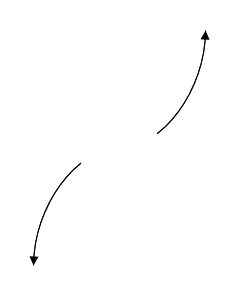
\includegraphics[width=0.3\textwidth]{../Figures/polyEndBehaviorCopyDB.png}
\end{center}\begin{enumerate}[label=\Alph*.]
\begin{multicols}{2}
\item 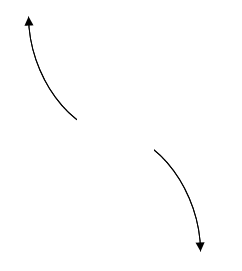
\includegraphics[width = 0.3\textwidth]{../Figures/polyEndBehaviorCopyAB.png}
\item 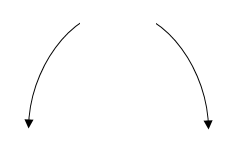
\includegraphics[width = 0.3\textwidth]{../Figures/polyEndBehaviorCopyBB.png}
\item 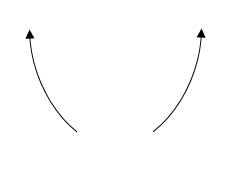
\includegraphics[width = 0.3\textwidth]{../Figures/polyEndBehaviorCopyCB.png}
\item 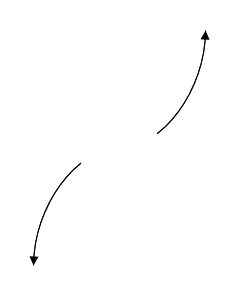
\includegraphics[width = 0.3\textwidth]{../Figures/polyEndBehaviorCopyDB.png}
\end{multicols}\item None of the above.\end{enumerate}
\textbf{General Comment:} Remember that end behavior is determined by the leading coefficient AND whether the \textbf{sum} of the multiplicities is positive or negative.
}
\litem{
Which of the following equations \textit{could} be of the graph presented below?

\begin{center}
    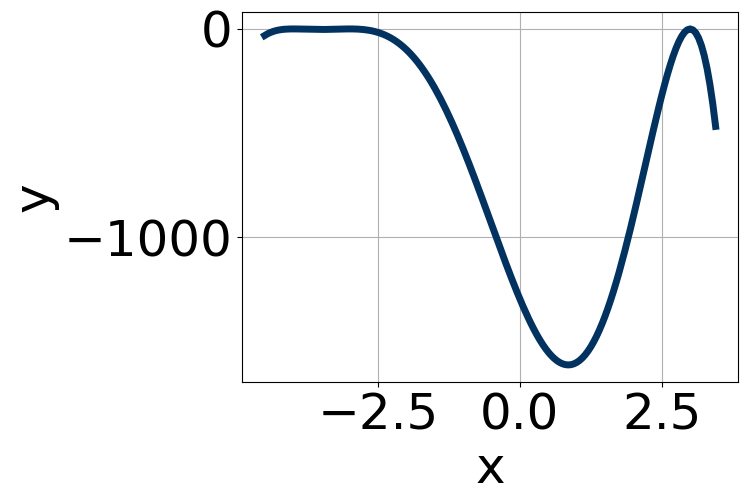
\includegraphics[width=0.5\textwidth]{../Figures/polyGraphToFunctionB.png}
\end{center}


The solution is \( -19x^{9} (x + 2)^{4} (x + 1)^{7} \), which is option C.\begin{enumerate}[label=\Alph*.]
\item \( -20x^{9} (x + 2)^{7} (x + 1)^{10} \)

The factor $-2$ should have an even power and the factor $-1$ should have an odd power.
\item \( 14x^{8} (x + 2)^{8} (x + 1)^{9} \)

The factor $x$ should have an odd power and the leading coefficient should be the opposite sign.
\item \( -19x^{9} (x + 2)^{4} (x + 1)^{7} \)

* This is the correct option.
\item \( 19x^{5} (x + 2)^{10} (x + 1)^{5} \)

This corresponds to the leading coefficient being the opposite value than it should be.
\item \( -18x^{7} (x + 2)^{4} (x + 1)^{10} \)

The factor $(x + 1)$ should have an odd power.
\end{enumerate}

\textbf{General Comment:} General Comments: Draw the x-axis to determine which zeros are touching (and so have even multiplicity) or cross (and have odd multiplicity).
}
\end{enumerate}

\end{document}